\section{Tool Architecture and Implementation}
\label{sec:implementation}

The Safety Annex is written in Java as a plug-in for the OSATE AADL toolset, which is built on Eclipse.  It is not designed as a stand-alone extension of the language, but works with behavioral contracts specified using the AGREE AADL annex~\cite{NFM2012:CoGaMiWhLaLu}. 
The architecture of the Safety Annex is shown in Figure~\ref{fig:plugin-arch}.

\begin{figure}
	\begin{center}
		%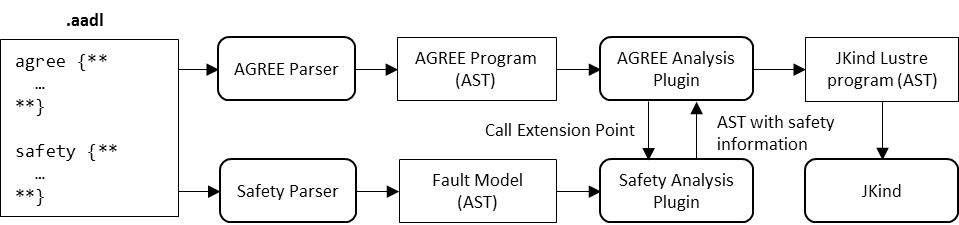
\includegraphics[trim=0 400 430 0,clip,width=0.85\textwidth]{images/arch.png}
		\includegraphics[width=\columnwidth]%.5\dimexpr\textwidth-2cm\relax]
	{images/arch.png}
	\end{center}
	\vspace{-0.2in}
	\caption{Safety Annex Plug-in Architecture}
	\label{fig:plugin-arch}
	\vspace{-0.2in}
\end{figure}

AGREE contracts are used to define the nominal behaviors of system components as {\em guarantees} that hold when {\em assumptions} about the values the component's environment are met. When an AADL model is annotated with AGREE contracts and the fault model is created using the Safety Annex, the model is transformed through AGREE into a Lustre model~\cite{Halbwachs91:IEEE} containing the behavioral extensions defined in the AGREE contracts for each system component. 

%This program is intercepted by the Safety Annex plugin and fault model information is added in two ways, depending on which form of fault analysis is being run. 

%\subsection{Verification in the Presence of Faults}
When performing fault analysis, the Safety Annex extends the AGREE contracts to allow faults to modify the behavior of component inputs and outputs. An example of a portion of an initial AGREE node and its extended contract is shown in Figure~\ref{fig:lustre}. The left column of the figure shows the nominal Lustre pump definition is shown with an AGREE contract on the output; and the right column shows the additional local variables for the fault (boxes 1 and 2), the assertion binding the fault value to the nominal value (boxes 3 and 4), and the fault node definition (box 5). Once augmented with fault information, the AGREE model (translated into the Lustre dataflow language~\cite{Halbwachs91:IEEE}) follows the standard translation path to the model checker JKind~\cite{2017arXiv171201222G}, an infinite-state model checker for safety properties. 

\begin{figure}[h!]
	\hspace*{-2cm}
	%\vspace{-0.3in} 
	\begin{center}
		%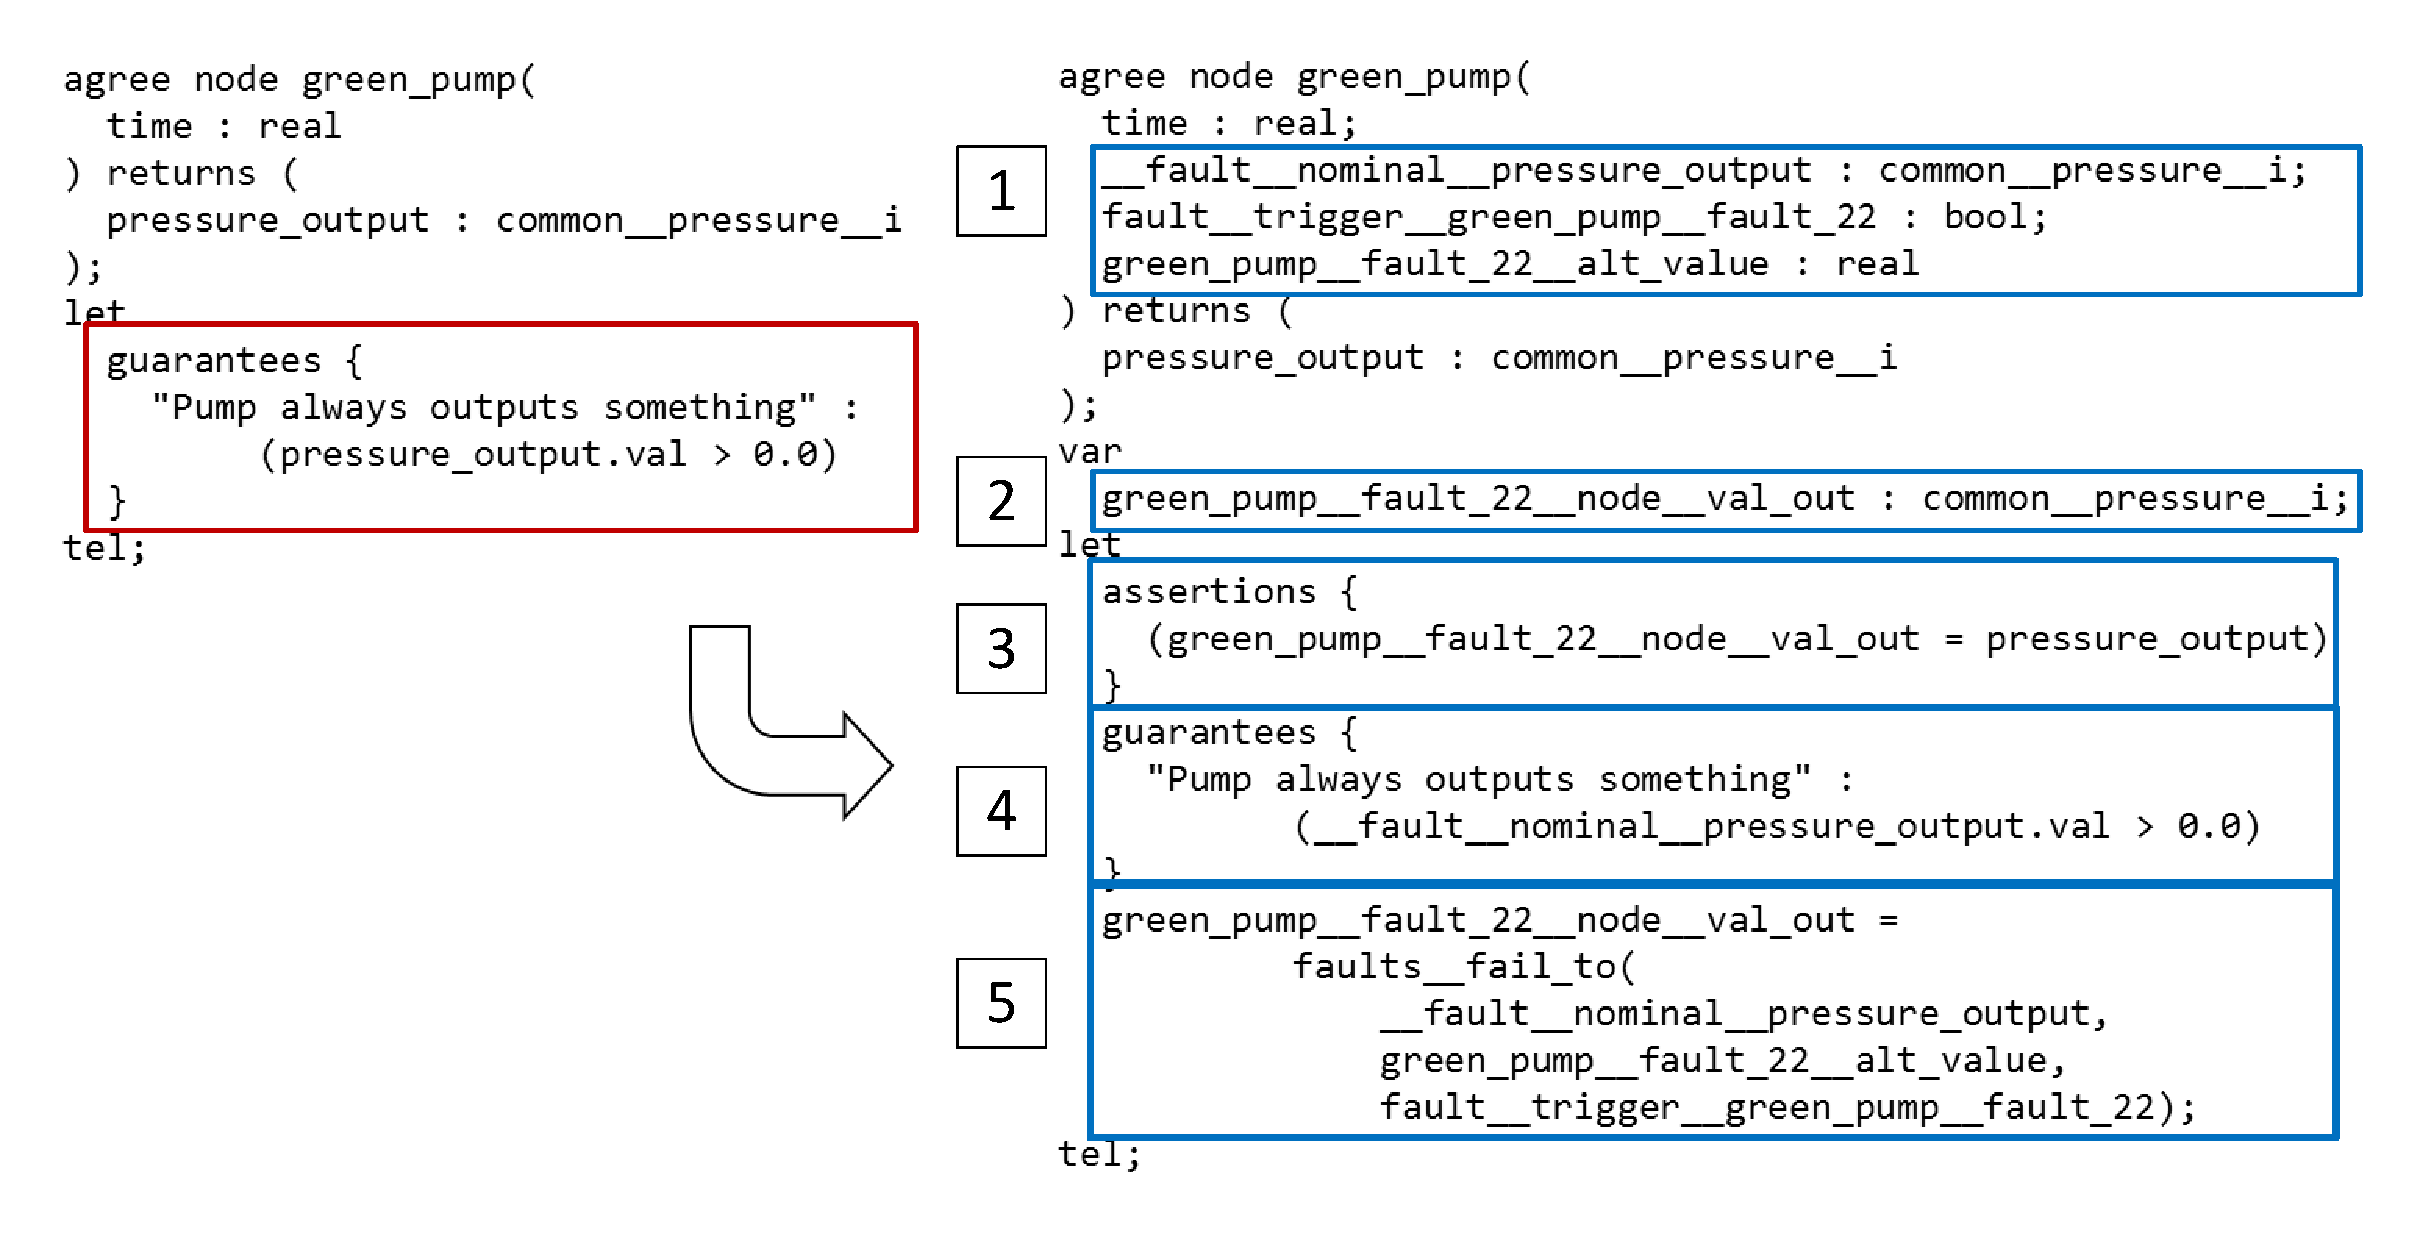
\includegraphics[trim=0 690 -10 70,clip,width=1.5\dimexpr\textwidth-2cm\relax]{images/lustre.pdf}
		\includegraphics[width=\columnwidth]%.5\dimexpr\textwidth-2cm\relax]
	{images/lustre.jpg}
		%\caption{Nominal AGREE node and its extension with faults}
		\caption{Nominal AGREE Node and Extension with Faults}
		\label{fig:lustre}
	\end{center}
	%\vspace{-0.3in}
\end{figure}

There are two different types of fault analysis that can be performed on a fault model. The Safety Annex plugin intercepts the AGREE program and add fault model information to the model depending on which form of fault analysis is being run.

\textbf{Verification in the Presence of Faults}: This analysis returns one counterexample when fault activation per the fault hypothesis can cause violation of a property. The augmentation from Safety Annex to the AGREE program includes traceability information so that when counterexamples are displayed to users, the active faults for each component are visualized.

\textbf{Generate Minimal Cut Sets}: This analysis returns all minimal cut sets that lead to the violation of a property, transformed from a full enumeration of all minimal set of model elements necessary for the inductive proofs of the property~\cite{Ghassabani2017EfficientGO,bendik2018online}.
\begin{comment}
\danielle{We will have to discuss this subsection. As is, it is not complete or sufficient for a full description, but I am not sure we want a full description since this stuff isn't published yet.} This analysis collects all minimal set of fault combinations that can cause violation of a property.
%\subsection{Generate Minimal Cut Sets}
Given a complex model, it is often useful to extract traceability information related to the proof, in other words, which portions of the model were necessary to construct the proof. An algorithm was introduced by Ghassabani, et. al. to provide Inductive Validity Cores (IVCs) as a way to determine which model elements are necessary for the inductive proofs of the safety properties for sequential systems~\cite{GhassabaniGW16}. Given a safety property of the system, a model checker can be invoked in order to construct a proof of the property. The IVC generation algorithm extracts traceability information from the proof process and returns a minimal set of the model elements required in order to prove the property. Later research extended this algorithm in order to produce all Minimal Inductive Validity Cores (All-MIVCs) to provide a full enumeration of all minimal set of model elements necessary for the inductive proofs of a safety property~\cite{Ghassabani2017EfficientGO}. 
\end{comment}



\begin{comment}
The IVC algorithm considers a constraint system consisting of the assumptions and contracts of system components and the negation of the safety property of interest (i.e. the top level event). It then collects what are called Minimal Unsatisfiable Subsets (MUSs) of this constraint system; these are the minimal explanations of the constraint systems infeasibility in terms of the \textit{negation} of the safety property. Equivalently, these are the minimal model elements necessary to proof the safety property. In section \ref{sec:definitions}, we show the formal definitions of IVCs in detail. 

In order to compositionally generate minimal cut sets, the all IVC algorithm is used~\cite{Ghassabani2017EfficientGO}, but instead of annotating the model with IVC elements consisting of only assumptions and contracts, we insert the faults in each layer constrained to false. The leaf nodes contribute only constrained faults to the IVC elements as shown in Figure~\ref{fig:ivcElements1}. 
\end{comment}
\begin{comment}
In this approach, we use the all MIVCs algorithm to consider a constraint system consisting of the negation of the top level safety property, the contracts of system components, as well as the faults in each layer constrained to false. It then collects what are called Minimal Unsatisfiable Subsets (MUSs) of this constraint system; these are the minimal explanations of the constraint systems infeasibility in terms of the \textit{negation} of the safety property. Equivalently, these are the minimal model elements necessary to proof the safety property. In section \ref{sec:definitions}, we show the formal definitions in detail. The leaf nodes contribute only constrained faults to the IVC elements as shown in Figure~\ref{fig:ivcElements1}. 

In the non-leaf layers of the program, both contracts and constrained faults are considered as shown in Figure~\ref{fig:ivcElements2}. The reason for this is that the contracts are used to prove the properties at the next highest level and are necessary for the verification of the properties. 

The all MIVCs algorithm returns the minimal set of these elements necessary to prove the properties. This equates to any contracts or inactive faults that must be present in order for the verification of properties in the model. From here, we perform a number of algorithms to transform all MIVCs into minimal cut sets (see Section~\ref{sec:theory} for more details on the transformation algorithms).
\end{comment}
\begin{comment}
\begin{figure}[h!]
	\hspace*{-2cm}
	\vspace{-0.1in} 
	\begin{center}
		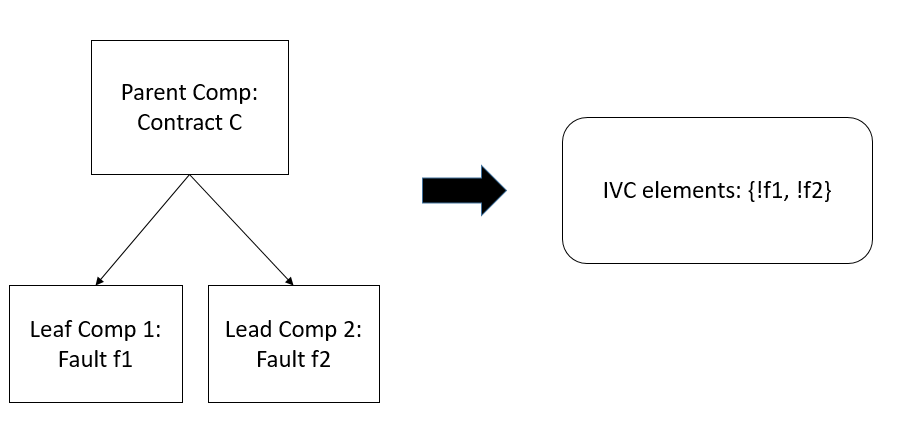
\includegraphics[scale=0.5]{images/ivcElements1.png}
	\caption{IVC Elements used for Consideration in a Leaf Layer of a System}
		\label{fig:ivcElements1}
	\end{center}
\end{figure}

\begin{figure}[h!]
	\hspace*{-2cm}
	\vspace{-0.1in} 
	\begin{center}
		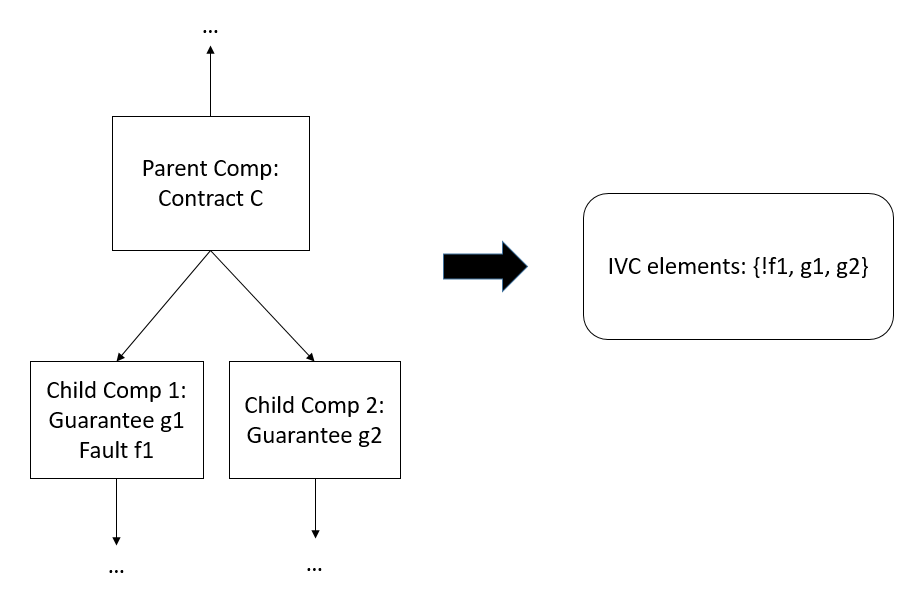
\includegraphics[scale=0.5]{images/ivcElements2.png}
	\caption{IVC Elements used for Consideration in a Middle Layer of a System}
		\label{fig:ivcElements2}
	\end{center}
\end{figure}
\end{comment}

\begin{comment}
The architecture of the Safety Annex is shown in Figure~\ref{fig:plugin-arch}.  It is written in Java as a plug-in for the OSATE AADL toolset, which is built on Eclipse.  It is not designed as a stand-alone extension of the language, but works with behavioral contracts specified in AGREE AADL annex and associated tools~\cite{NFM2012:CoGaMiWhLaLu}.  AGREE allows {\em assume-guarantee} behavioral contracts to be added to AADL components.  The language used for contract specification is based on the Lustre dataflow language~\cite{Halbwachs91:IEEE}. AGREE improves scalability of formal verification to large systems by decomposing the analysis of a complex system architecture into a collection of smaller verification tasks that correspond to the structure of the architecture.

\begin{figure}
	\begin{center}
		%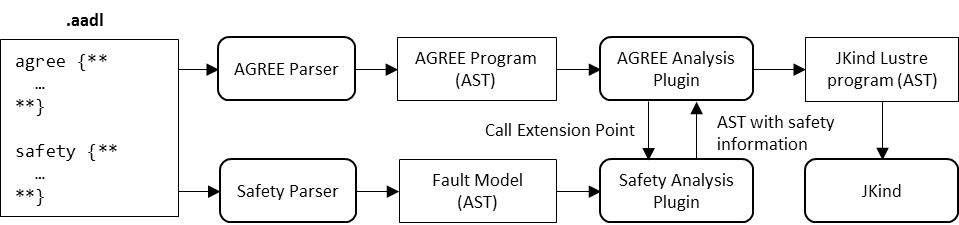
\includegraphics[trim=0 400 430 0,clip,width=0.85\textwidth]{images/arch.png}
		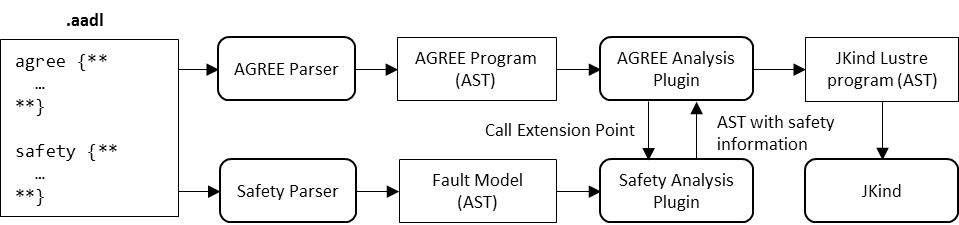
\includegraphics[width=.9\textwidth]{images/arch.png}
	\end{center}
	\vspace{-0.2in}
	\caption{Safety Annex Plug-in Architecture}
	\label{fig:plugin-arch}
\end{figure}

AGREE contracts are used to define the nominal behaviors of system components as {\em guarantees} that hold when {\em assumptions} about the values the component's environment are met.  The Safety Annex extends these contracts to allow faults to modify the behavior of component inputs and outputs.  To support these extensions, AGREE implements an Eclipse extension point interface that allows other plug-ins to modify the generated abstract syntax tree (AST) prior to its submission to the solver.  If the Safety Annex is enabled, these faults are added to the AGREE contract and, when triggered, override the nominal guarantees provided by the component.  

An example of a portion of an initial AGREE node and its extended contract is shown in Figure~\ref{fig:lustre}. 
In the left column of the figure, the nominal Lustre pump definition is shown with an AGREE contract on the output. In the right column, the additional local variables for the fault are seen in boxes 1 and 2, the assertion binding the fault value to the nominal value is seen in boxes 3 and 4, and the fault node definition is given in box 5. 

\begin{figure}[h!]
	\hspace*{-2cm}
	\vspace{-0.3in} 
	\begin{center}
		%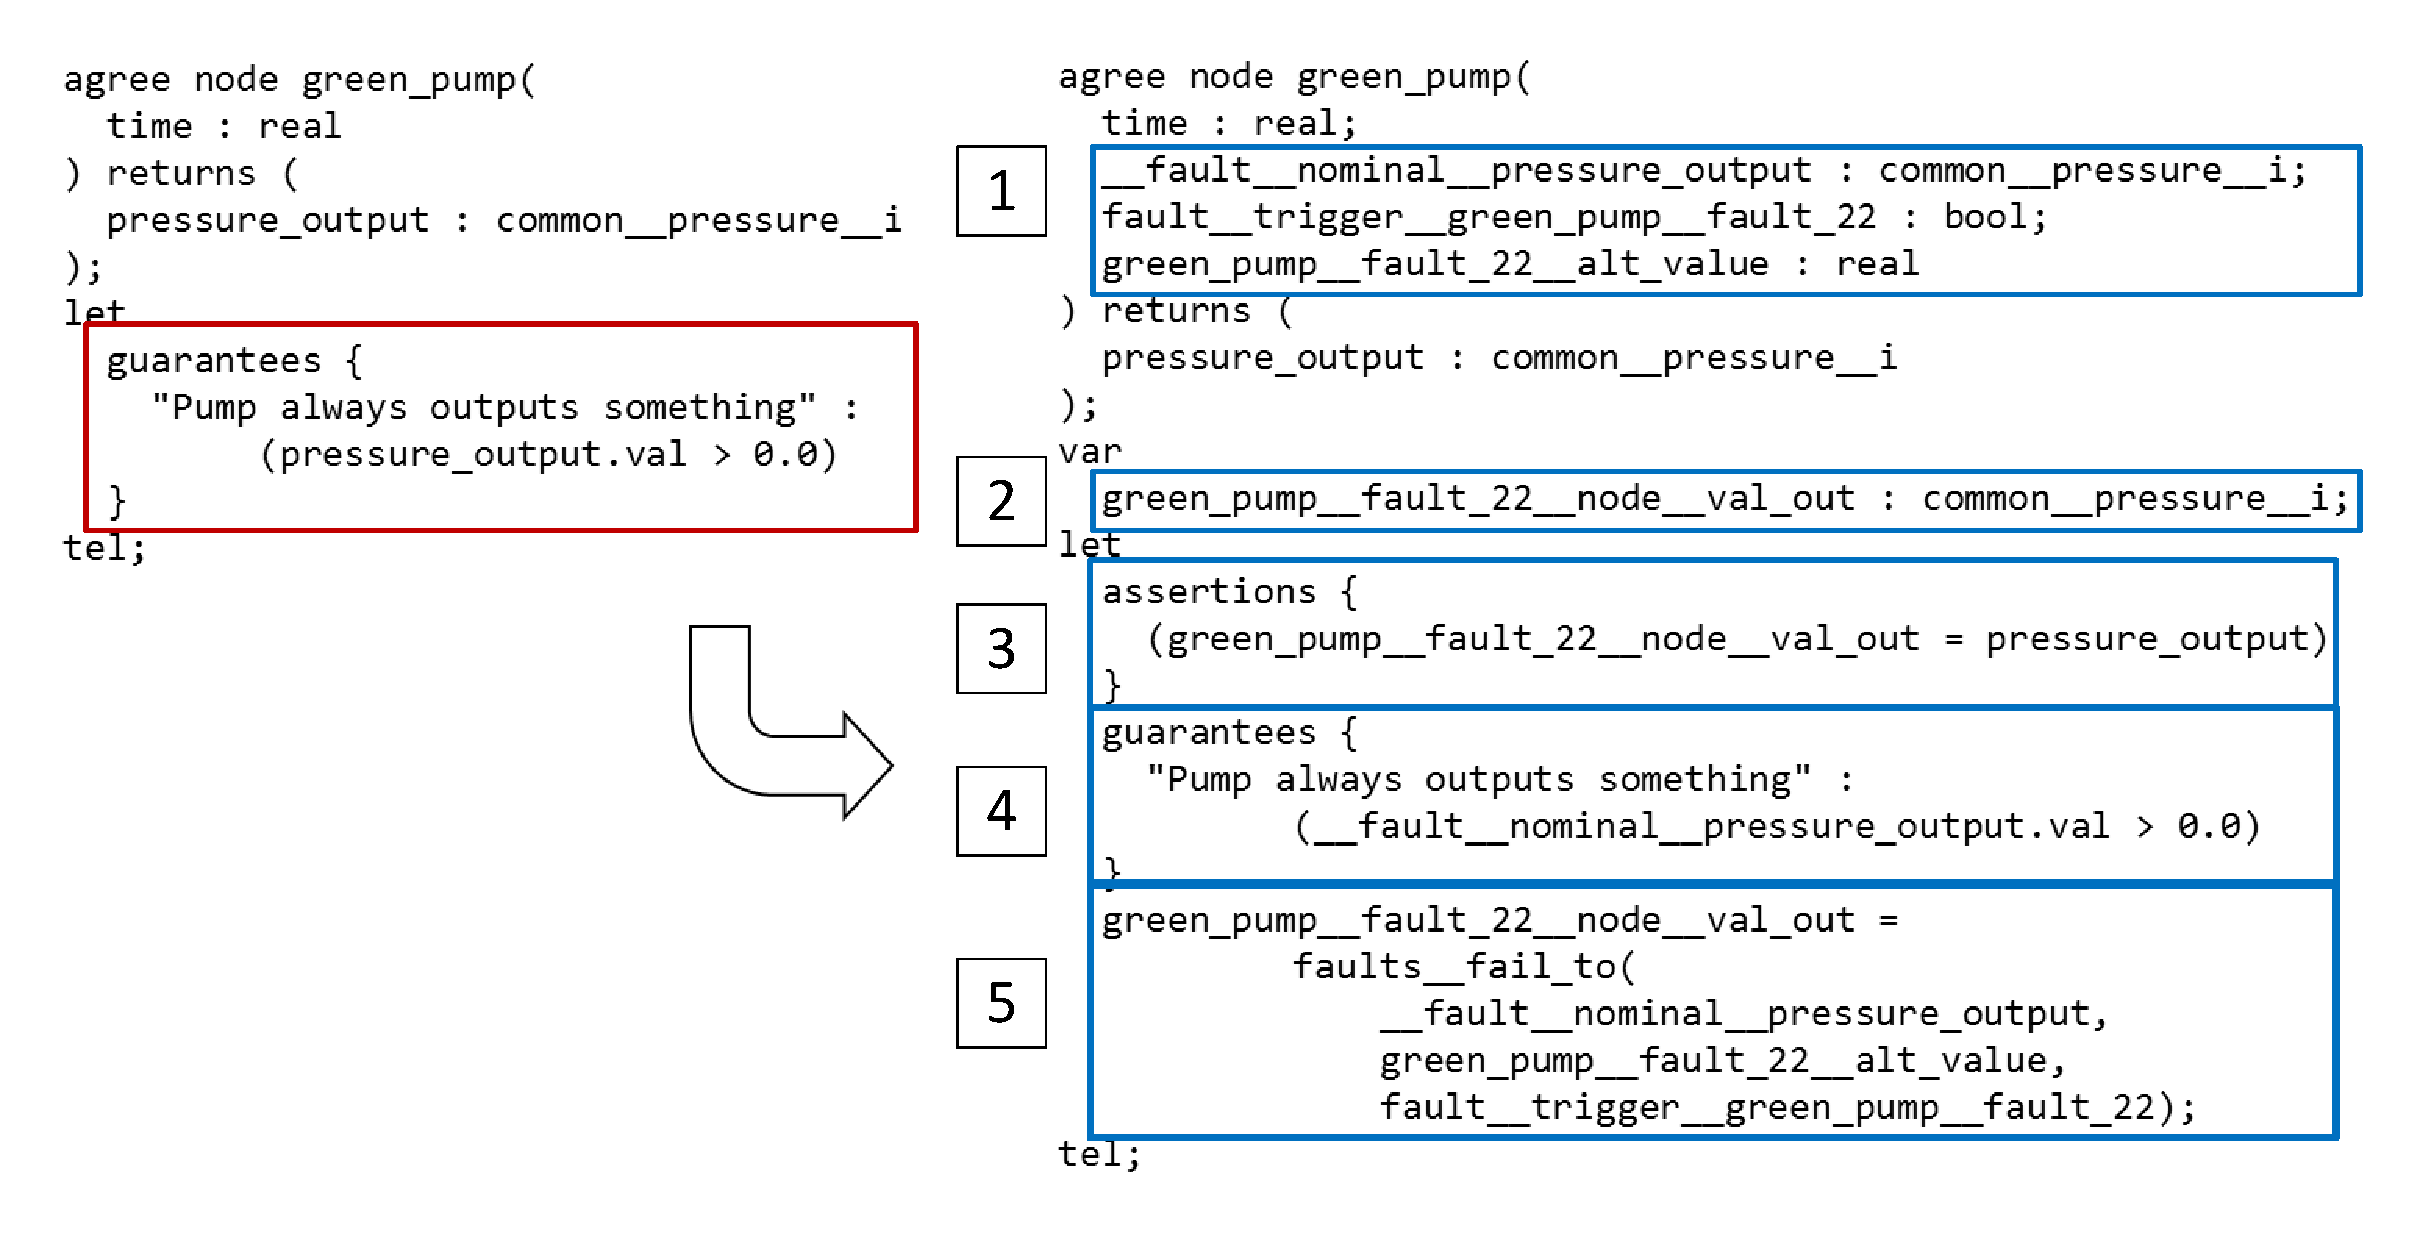
\includegraphics[trim=0 690 -10 70,clip,width=1.5\dimexpr\textwidth-2cm\relax]{images/lustre.pdf}
		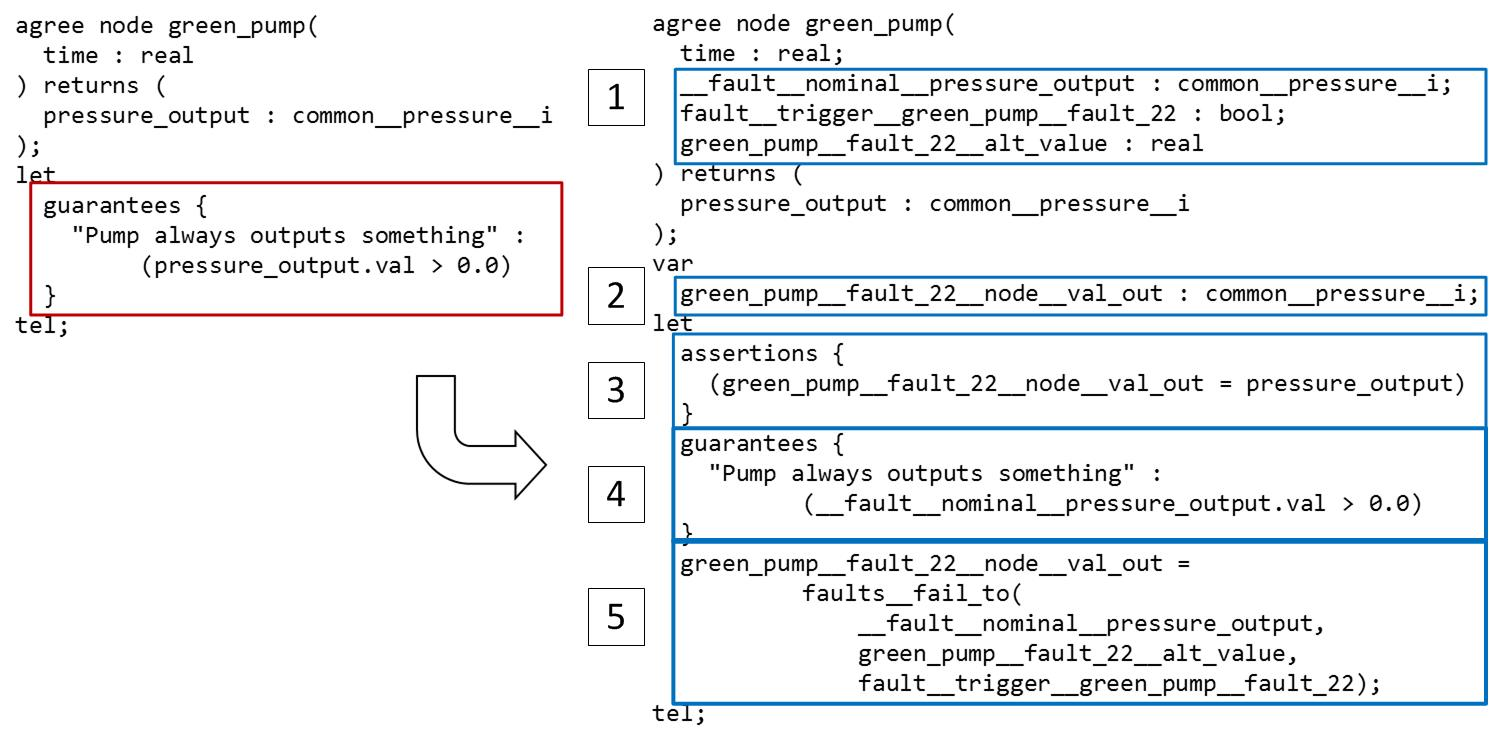
\includegraphics[scale=0.3]{images/lustre.jpg}
		\caption{Nominal AGREE node and its extension with faults}
		\label{fig:lustre}
	\end{center}
	\vspace{-0.3in}
\end{figure}


Once augmented with fault information, the AGREE model follows the standard translation path to the model checker JKind~\cite{2017arXiv171201222G}, an infinite-state model checker for safety properties.  The augmentation includes traceability information so that when counterexamples are displayed to users, the active faults for each component are visualized.

The architecture of the Safety Annex is shown in Figure~\ref{fig:plugin-arch}.  It is written in Java as a plug-in for the OSATE AADL toolset, which is built on Eclipse.  It is not designed as a stand-alone extension of the language, but works with behavioral contracts specified in AGREE AADL annex and associated tools~\cite{NFM2012:CoGaMiWhLaLu}.  AGREE allows {\em assume-guarantee} behavioral contracts to be added to AADL components.  The language used for contract specification is based on the Lustre dataflow language~\cite{Halbwachs91:IEEE}. AGREE improves scalability of formal verification to large systems by decomposing the analysis of a complex system architecture into a collection of smaller verification tasks that correspond to the structure of the architecture.

\begin{figure}
	\begin{center}
		%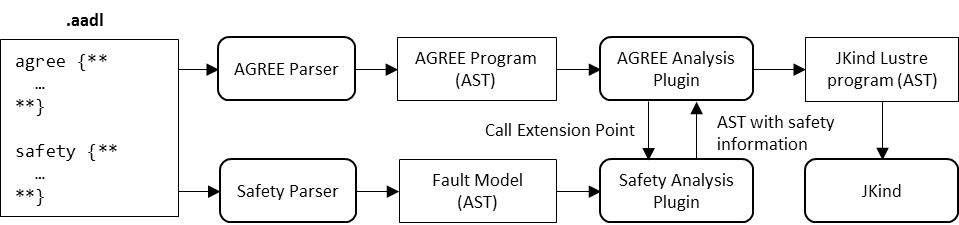
\includegraphics[trim=0 400 430 0,clip,width=0.85\textwidth]{images/arch.png}
		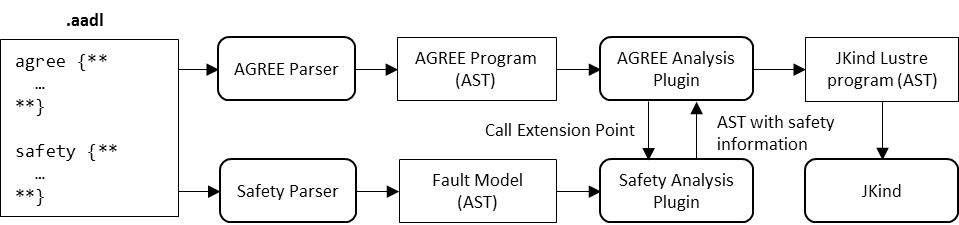
\includegraphics[width=.9\textwidth]{images/arch.png}
	\end{center}
	\vspace{-0.2in}
	\caption{Safety Annex Plug-in Architecture}
	\label{fig:plugin-arch}
\end{figure}

AGREE contracts are used to define the nominal behaviors of system components as {\em guarantees} that hold when {\em assumptions} about the values the component's environment are met.  The Safety Annex extends these contracts to allow faults to modify the behavior of component inputs and outputs.  To support these extensions, AGREE implements an Eclipse extension point interface that allows other plug-ins to modify the generated abstract syntax tree (AST) prior to its submission to the solver.  If the Safety Annex is enabled, these faults are added to the AGREE contract and, when triggered, override the nominal guarantees provided by the component.  

An example of a portion of an initial AGREE node and its extended contract is shown in Figure~\ref{fig:lustre}.  %The \texttt{\_\_fault} variables and declarations are added to allow the contract to override the nominal behavioral constraints (provided by guarantees) on outputs.  In the Lustre language, \texttt{assertion}s are constraints that are assumed to hold in the transition system. 
In the left column of the figure, the nominal Lustre pump definition is shown with an AGREE contract on the output. In the right column, the additional local variables for the fault are seen in boxes 1 and 2, the assertion binding the fault value to the nominal value is seen in boxes 3 and 4, and the fault node definition is given in box 5. 

%A  benefit of utilizing the AGREE behavioral annex is the ability to perform both monolithic and compositional analysis on the nominal model. AGREE allows {\em assume-guarantee} behavioral contracts to be added to AADL components.  The language used for contract specification is based on the Lustre dataflow language~\cite{Halbwachs91:IEEE} and the nominal model (AADL model annotated with AGREE contracts) is translated into Lustre before being sent to the JKind model checker for verification\cite{2017arXiv171201222G}. 

%When a user selects to run the fault analysis during verification, the AGREE contracts are automatically extended in Lustre in order to allow faults to modify the behavior of component outputs. These injections into the Lustre model are shown in Figure~\ref{fig:lustre}. 

\begin{figure}[h!]
	\hspace*{-2cm}
	\vspace{-0.3in} 
	\begin{center}
		%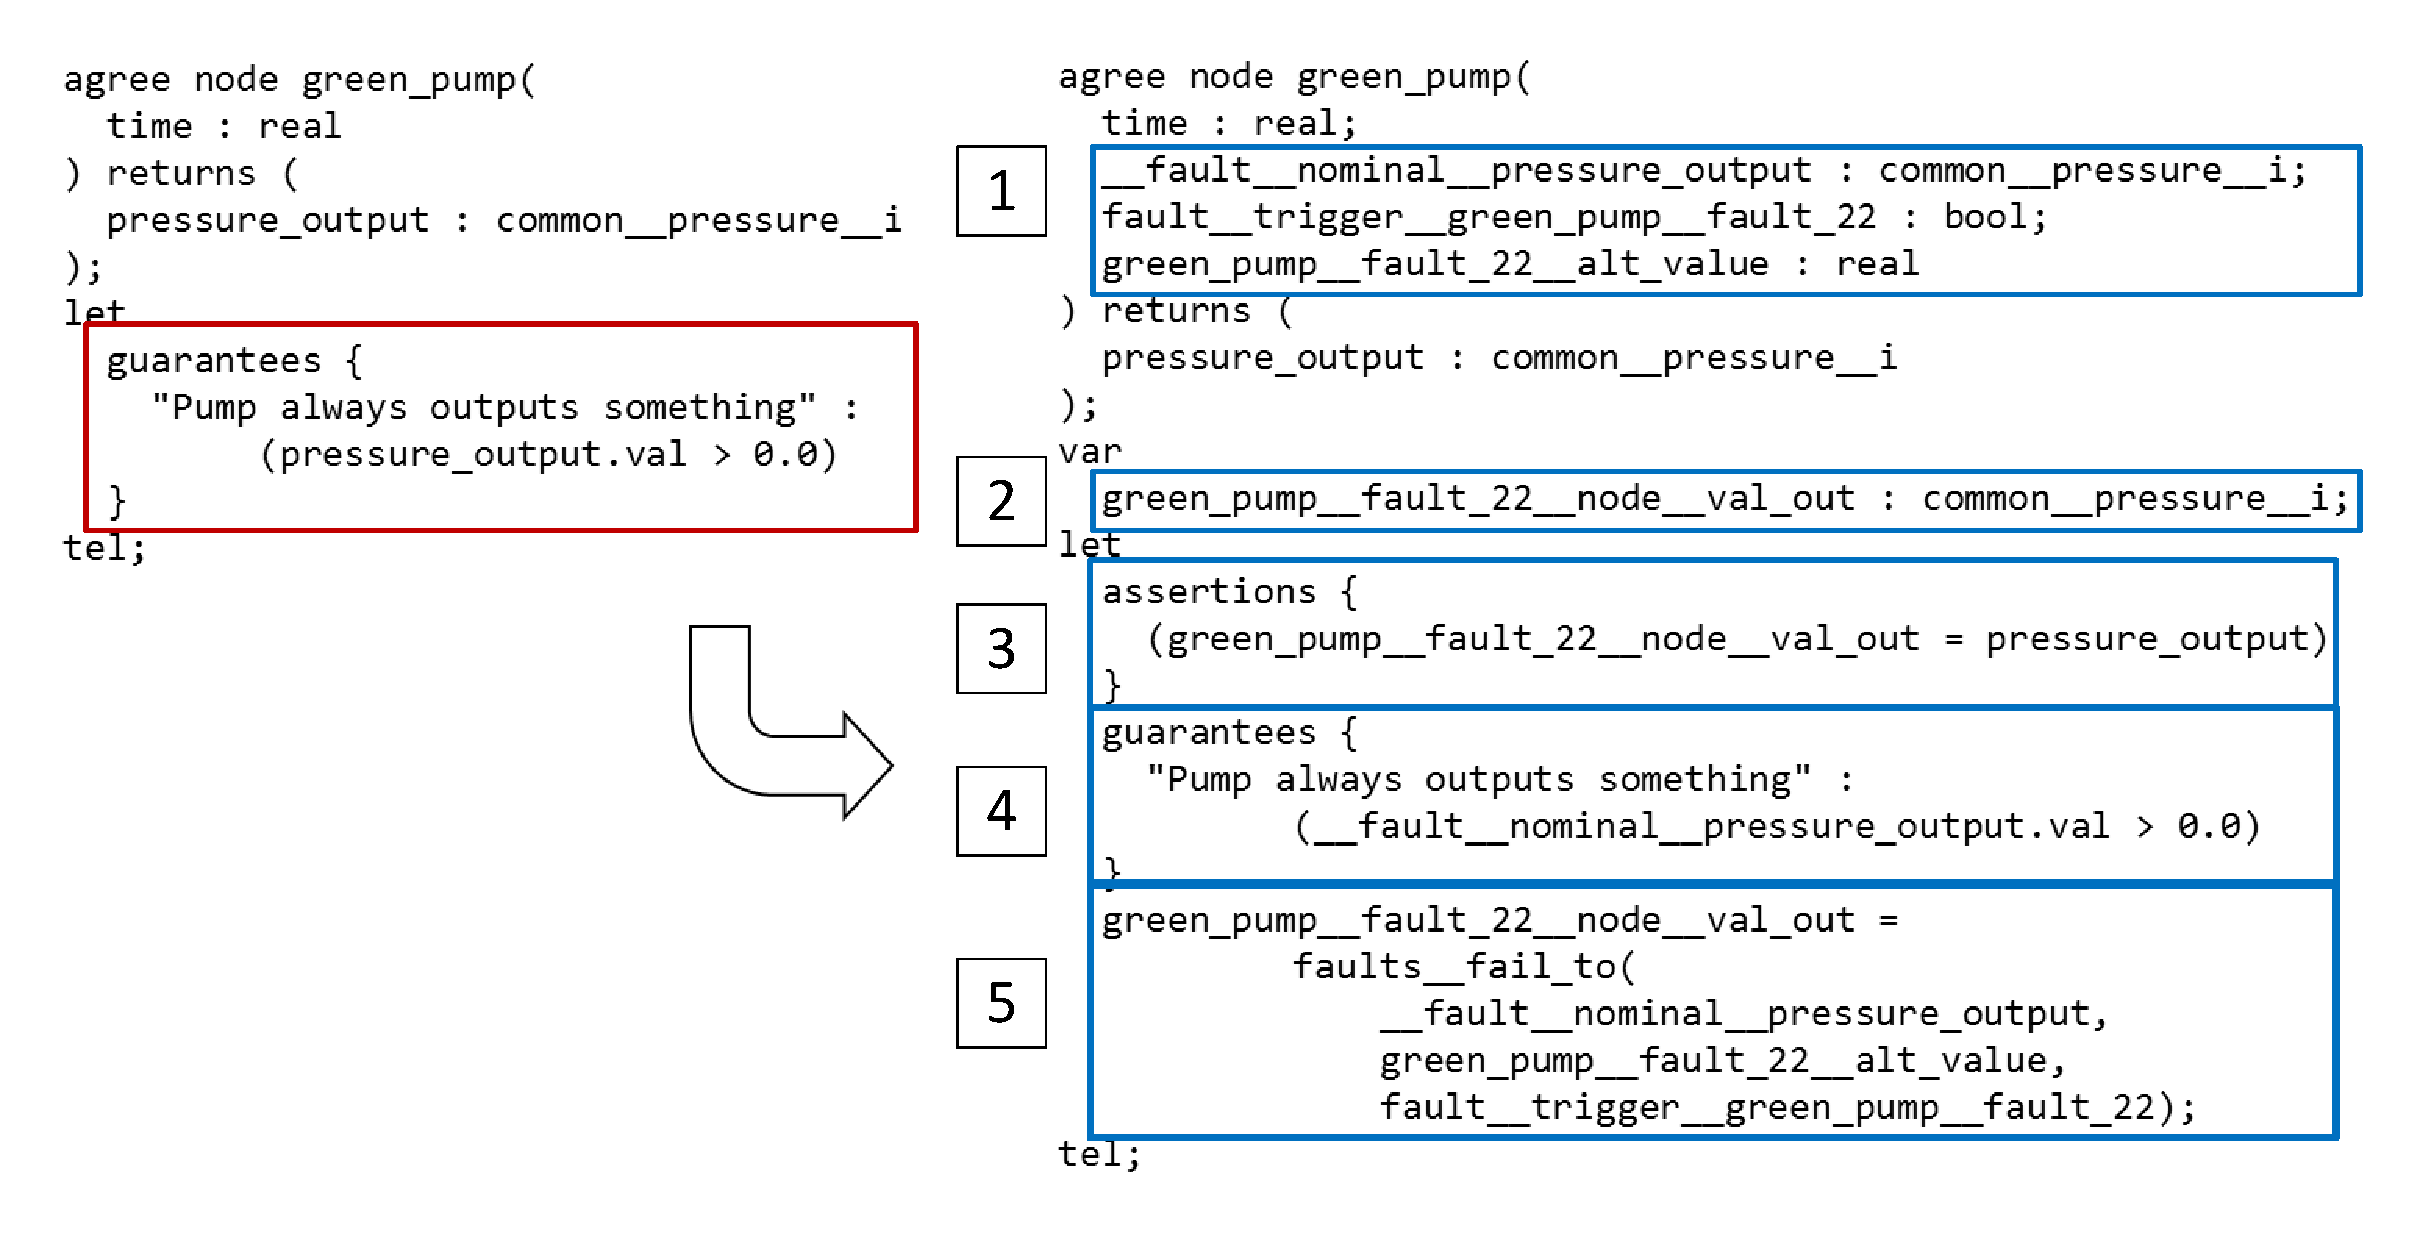
\includegraphics[trim=0 690 -10 70,clip,width=1.5\dimexpr\textwidth-2cm\relax]{images/lustre.pdf}
		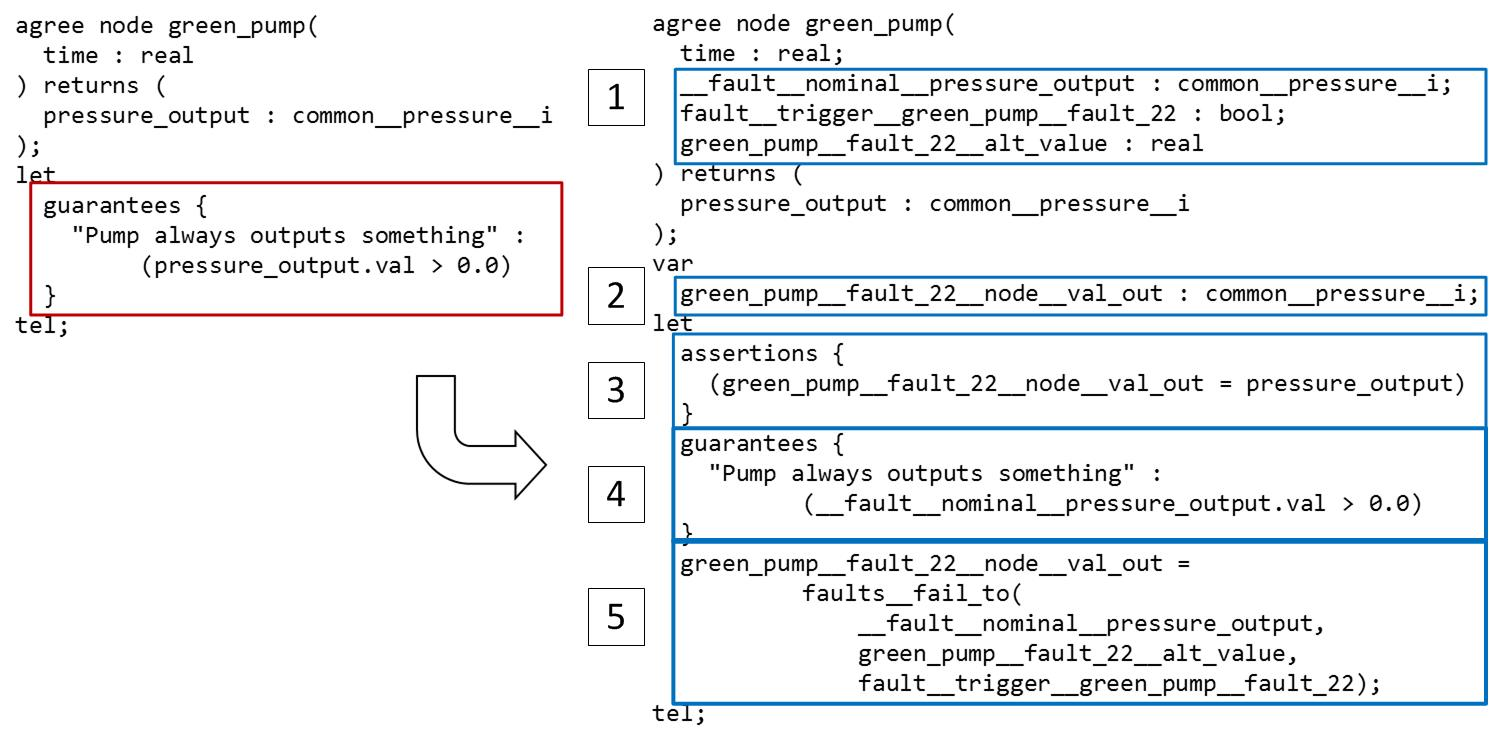
\includegraphics[scale=0.3]{images/lustre.jpg}
		\caption{Nominal AGREE node and its extension with faults}
		\label{fig:lustre}
	\end{center}
	\vspace{-0.3in}
\end{figure}

\begin{comment}
\begin{figure}
	\vspace{-0.1in}
	%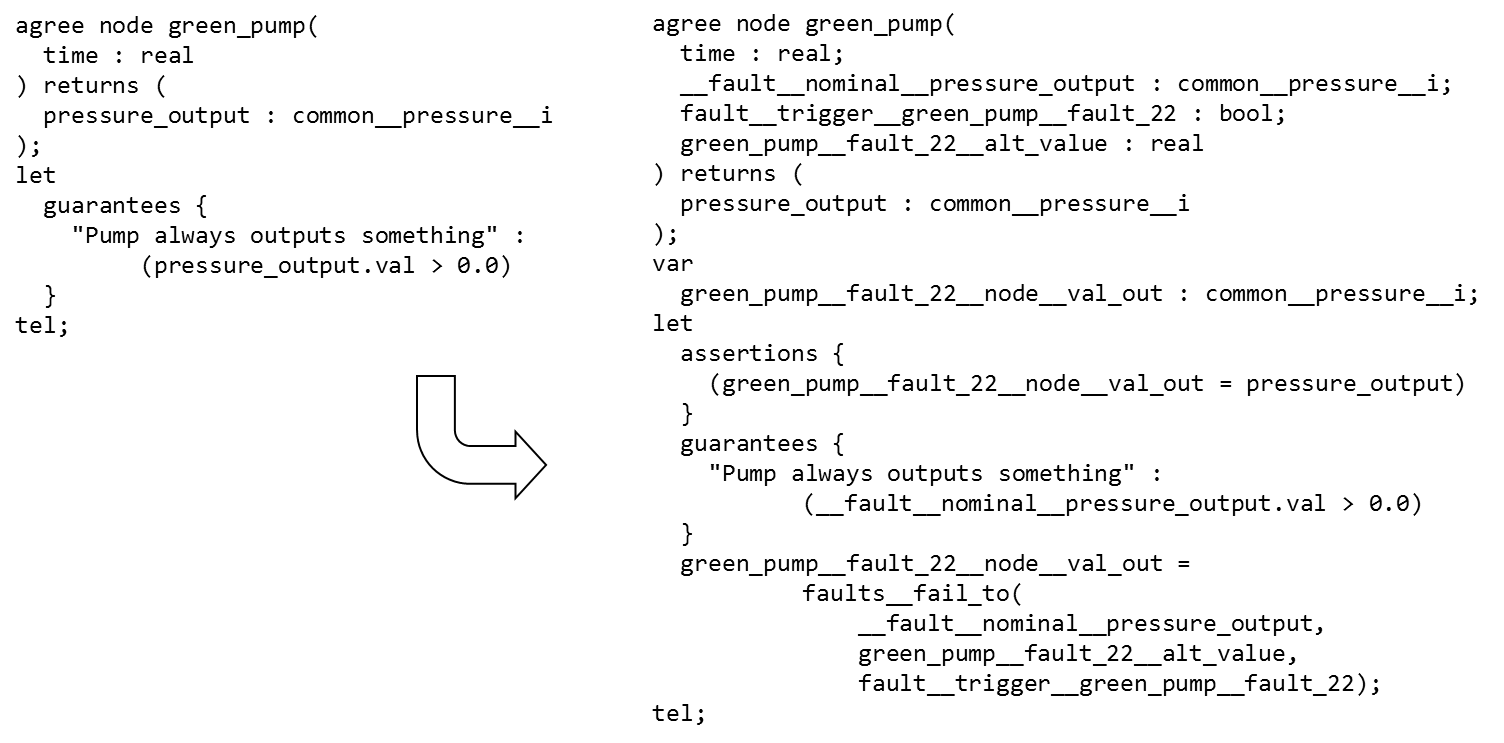
\includegraphics[trim=30 150 120 10,clip,width=\textwidth]{images/sample_code.png}
	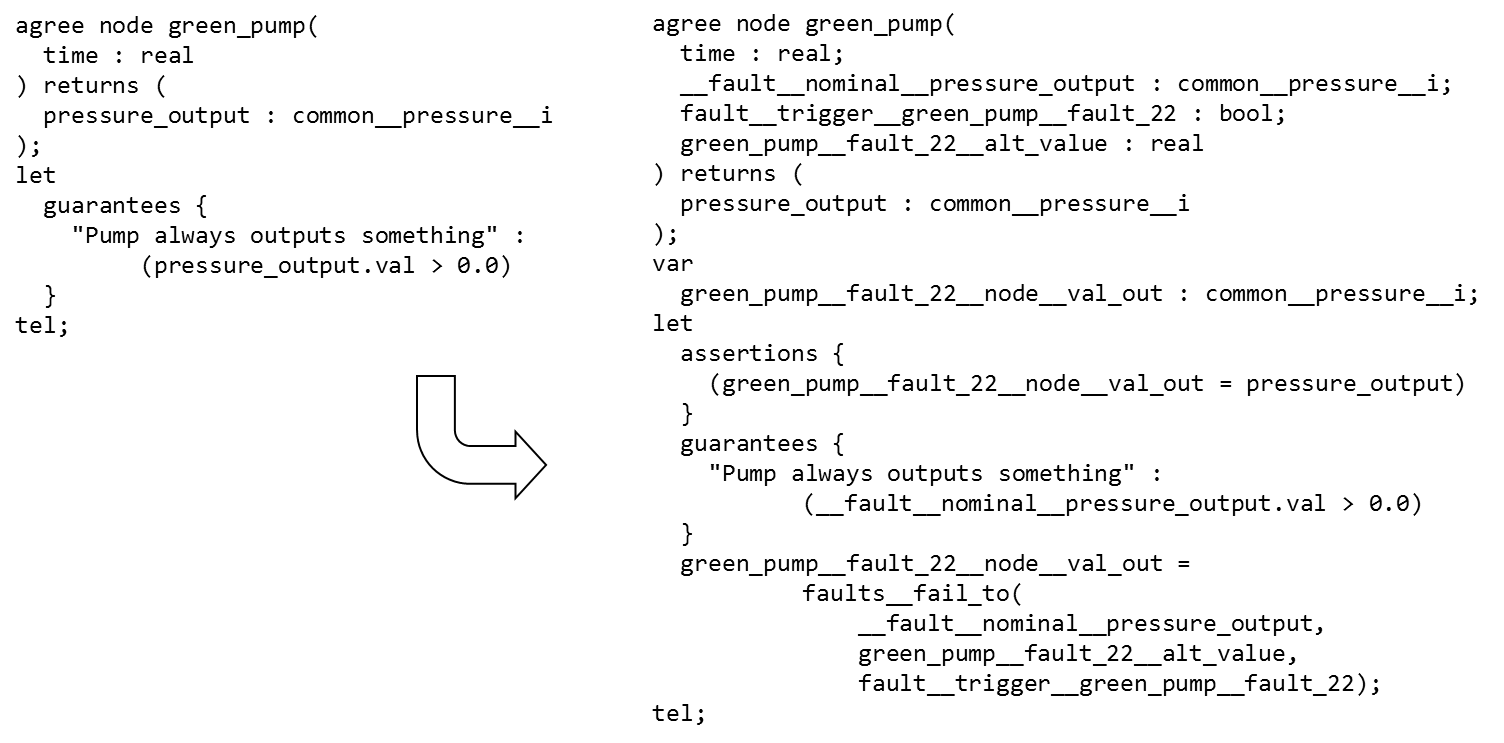
\includegraphics[width=\textwidth]{images/sample_code.png}
	\vspace{-0.3in}
	\caption{Nominal AGREE node and its extension with faults}
	\label{fig:comp}
\end{figure}
\end{comment}
%An annotation in the AADL model determines the fault hypothesis.  This may specify either a maximum number of faults that can be active at any point in execution (typically one or two), or that only faults whose probability of simultaneous occurrence is above some probability threshold should be considered. In the former case, we assert that the sum of the true {\em fault\_\_trigger} variables is below some integer threshold.  In the latter, we determine all combinations of faults whose probabilities are above the specified probability threshold, and describe this as a proposition over {\em fault\_\_trigger} variables.
%
%With the introduction of dependent faults, active faults are divided into two categories: independently active (activated by its own triggering event) and dependently active (activated when the faults they depend on become active). The top level fault hypothesis applies to independently active faults. Faulty behaviors augment nominal behaviors whenever their corresponding faults are active (either independently active or dependently active).

%Once augmented with fault information, the AGREE model follows the standard translation path to the model checker JKind~\cite{2017arXiv171201222G}, an infinite-state model checker for safety properties.  The augmentation includes traceability information so that when counterexamples are displayed to users, the active faults for each component are visualized.


%For fault analysis, we separate the possible analyses available to users into two distinct actions and describe them here.
